\documentclass[tikz,border=2]{standalone}
\usetikzlibrary{shadows,arrows,shapes,positioning,calc,backgrounds,fit}
% FIGURES
\usepackage{graphicx}
\graphicspath{./figs}
\usepackage{grffile} % to set right names of files
\usepackage{colortbl}
\usepackage{array}
\usepackage{multirow}
\pdfpageattr {/Group << /S /Transparency /I true /CS /DeviceRGB>>}
\newcommand{\parnode}[1]{\parbox{3cm}{\centering #1}}
\DeclareGraphicsRule{.ai}{pdf}{.ai}{}
% Define the layers to draw the diagram
%

\begin{document}
\begin{tikzpicture}
    \node (current) [label=below:a] {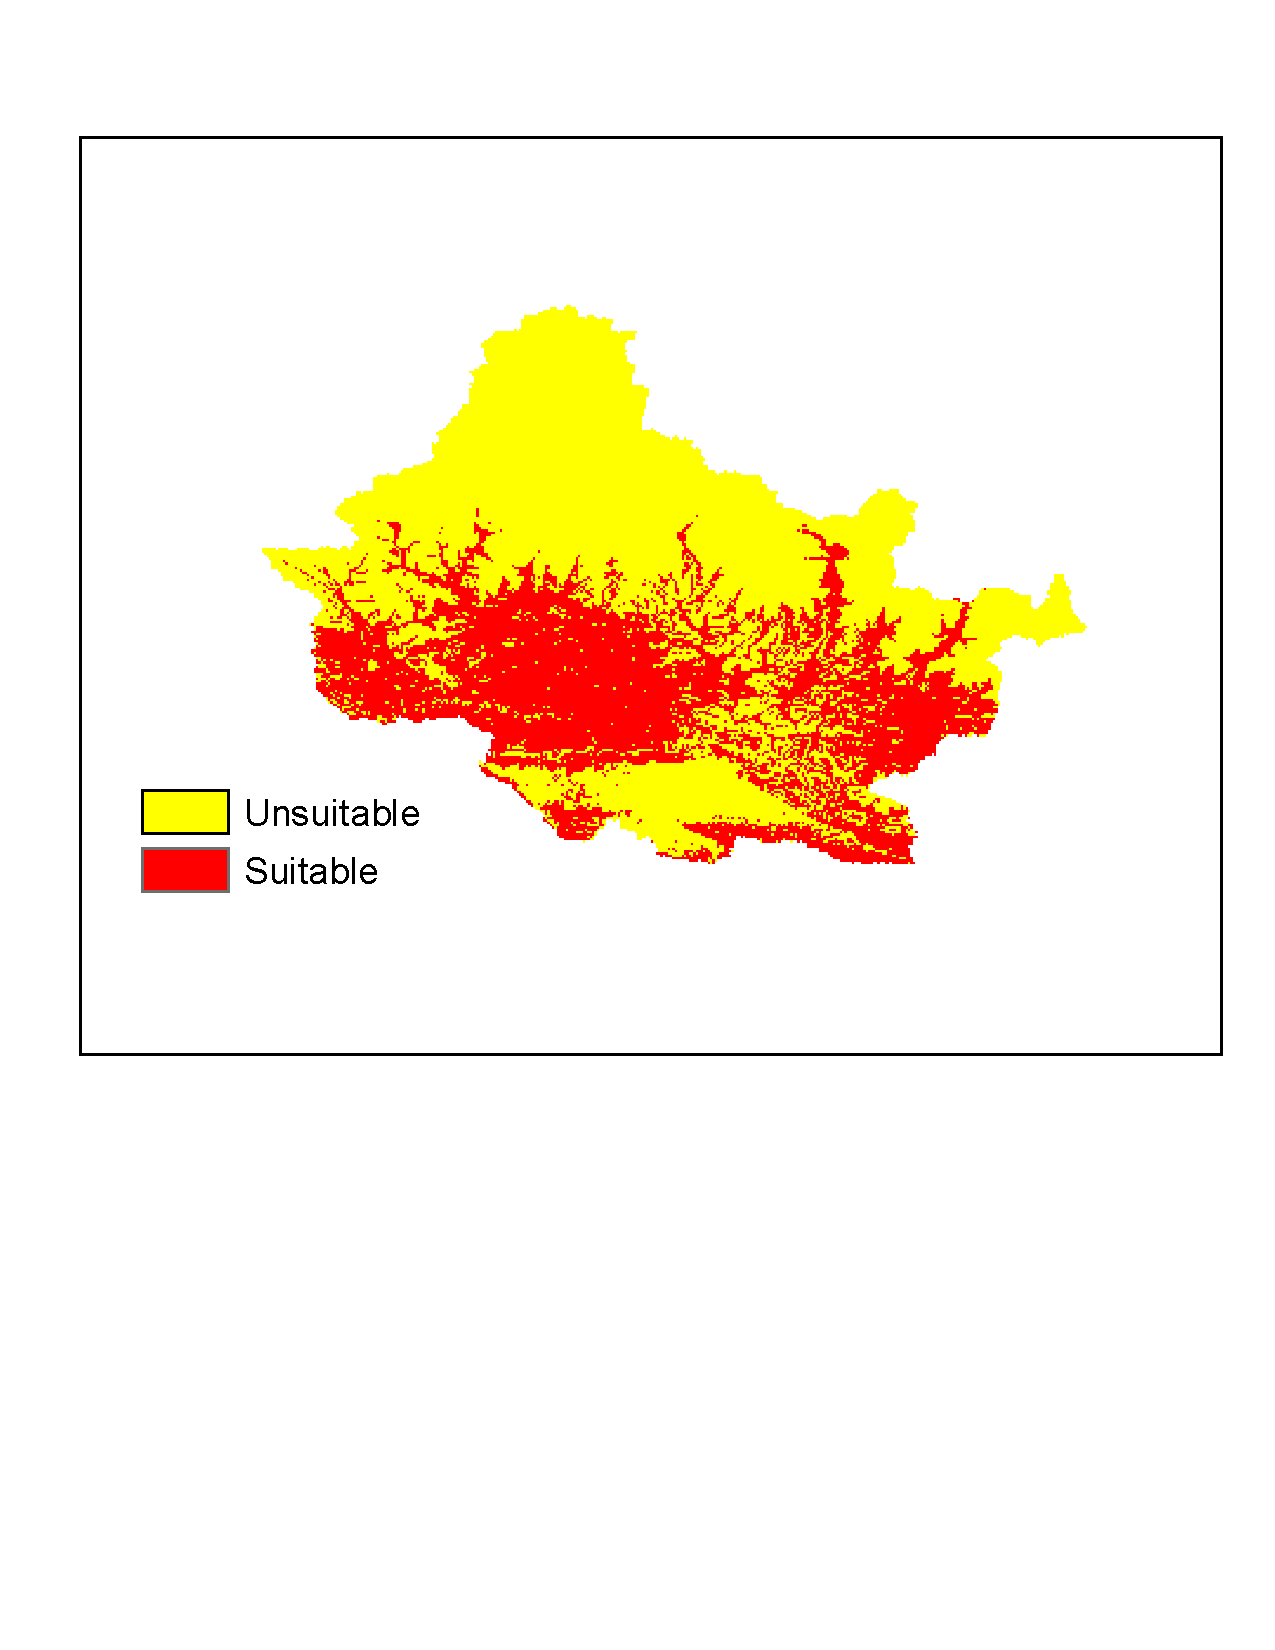
\includegraphics[trim=60 350 60 140,clip,width=5cm]{Current.pdf}};
    \node (2650) at (-2,-3) [label=below:b] {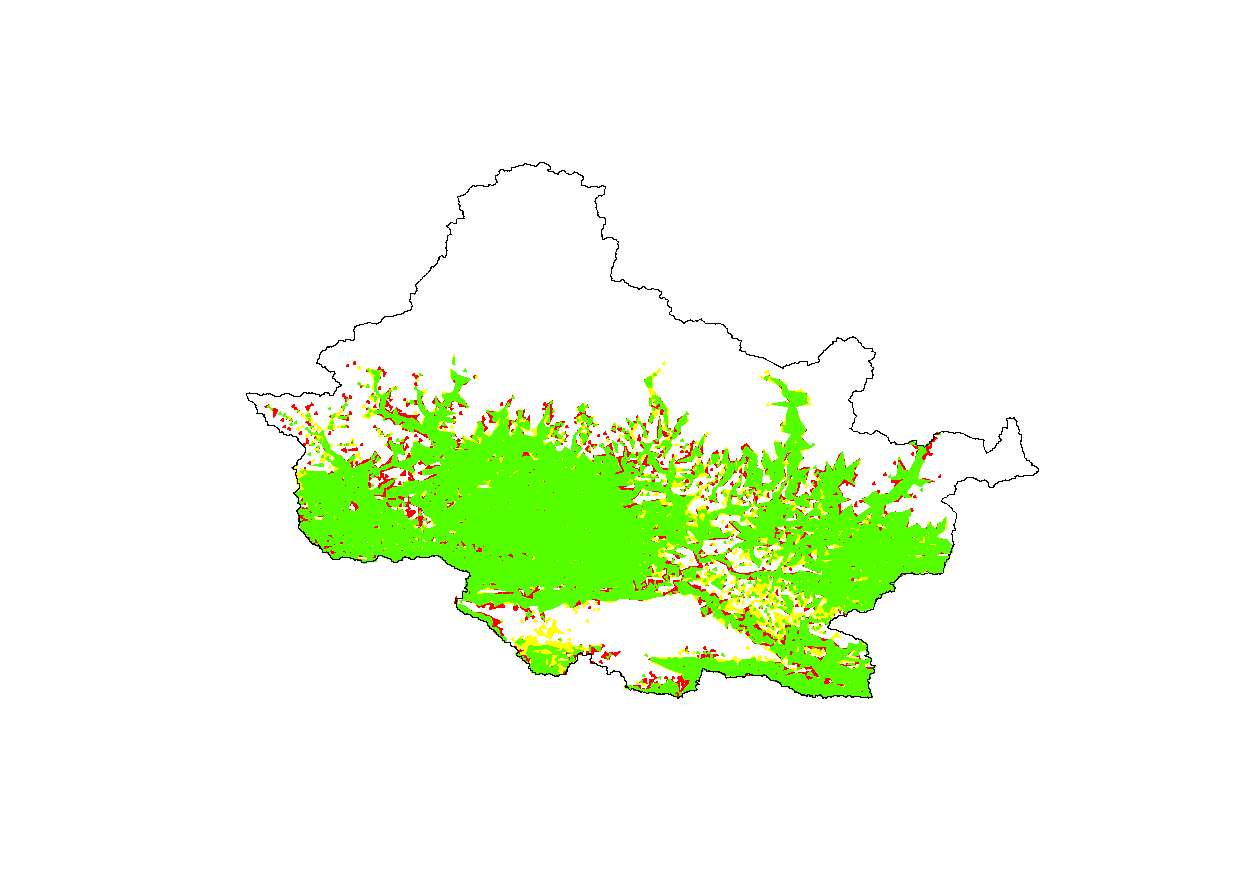
\includegraphics[trim=0 40 0 20,clip,width=5cm]{2650.pdf}};
    \node (2670) at (2,-3) [label=below:c] {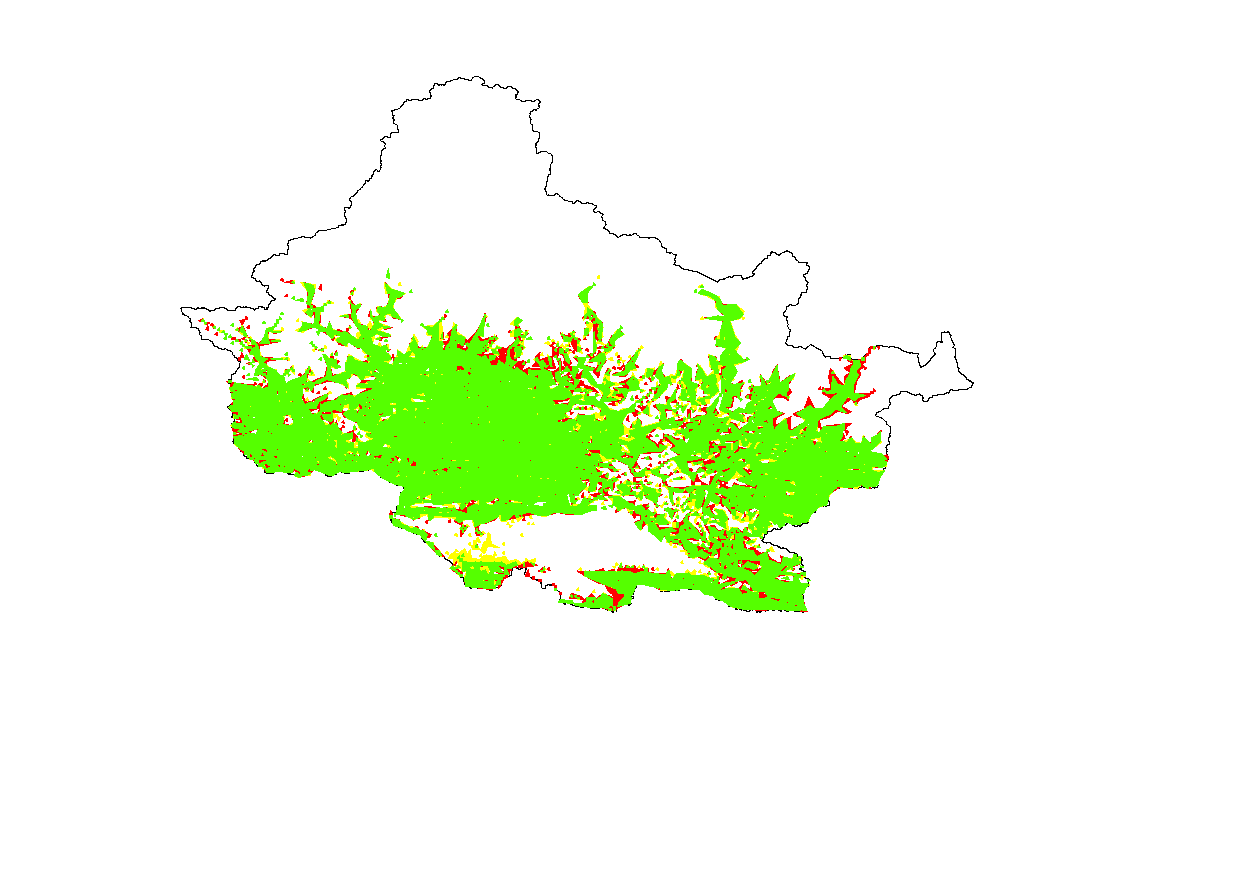
\includegraphics[trim=0 80 0 0,clip,width=5cm]{2670.pdf}};
    \node (4550) at (-1.6,-7) [label=below:d] {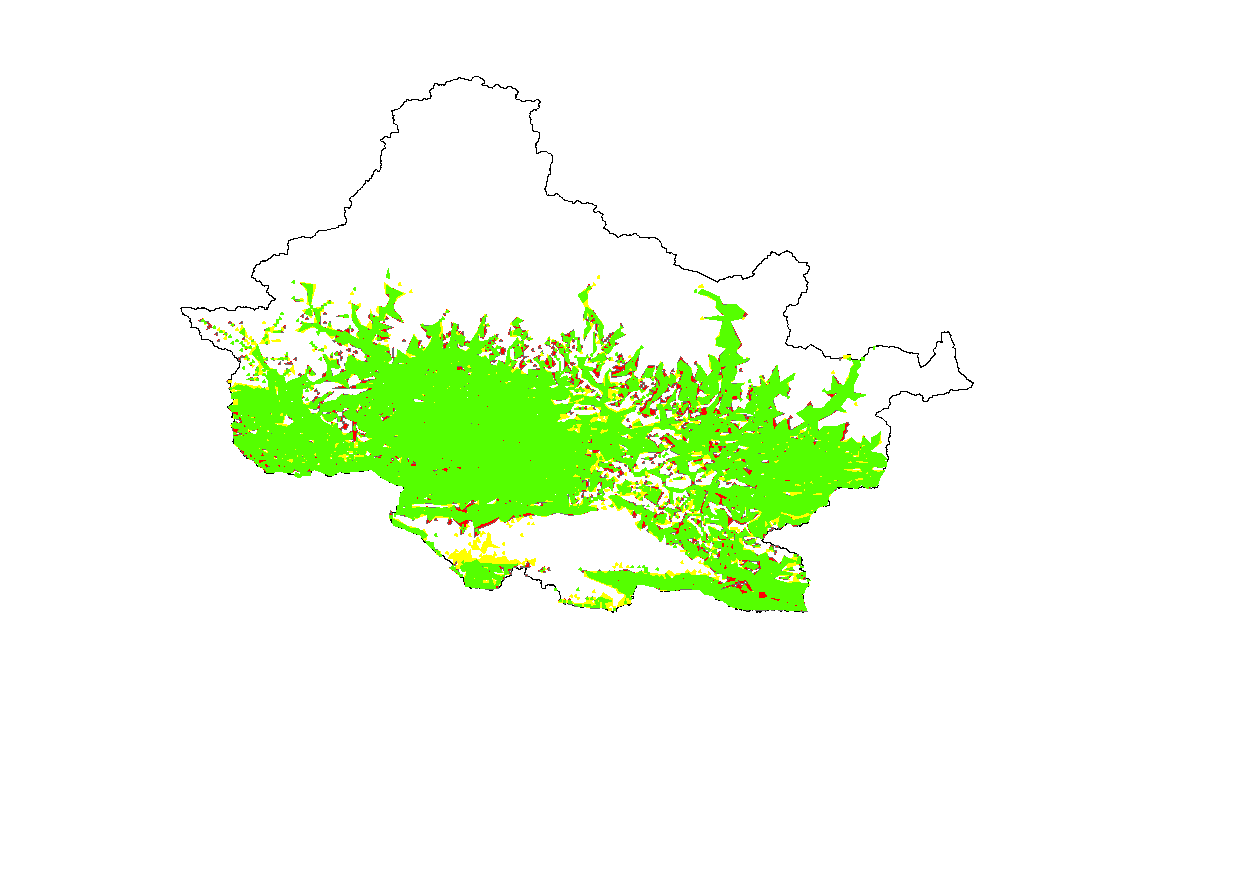
\includegraphics[trim=0 80 0 0,clip,width=5cm]{4550.pdf}};
    \node (4570) at (2,-7) [label=below:e] {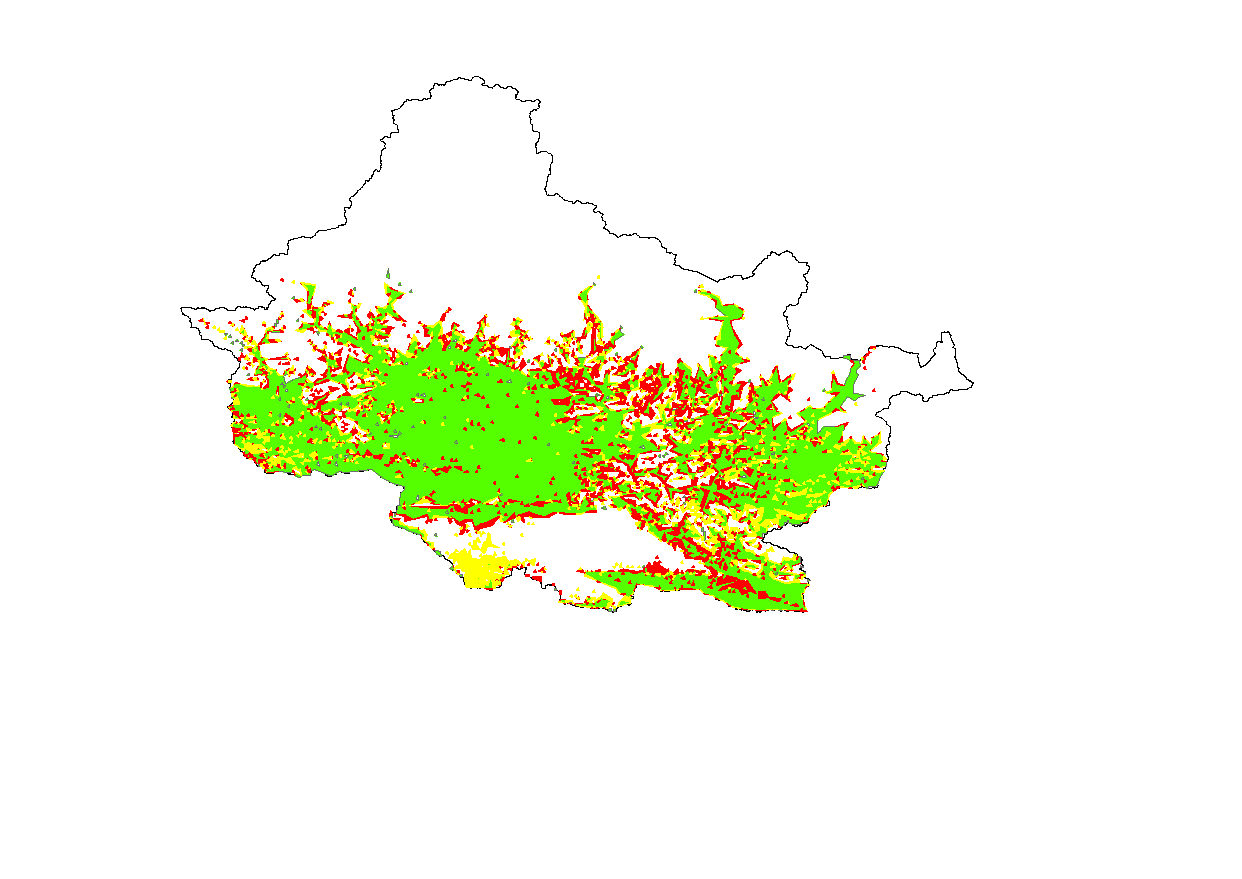
\includegraphics[trim=0 80 0 0,clip,width=5cm]{4570.pdf}};
    \node (8550.pdf) at (-1.6,-11) [label=below:f] {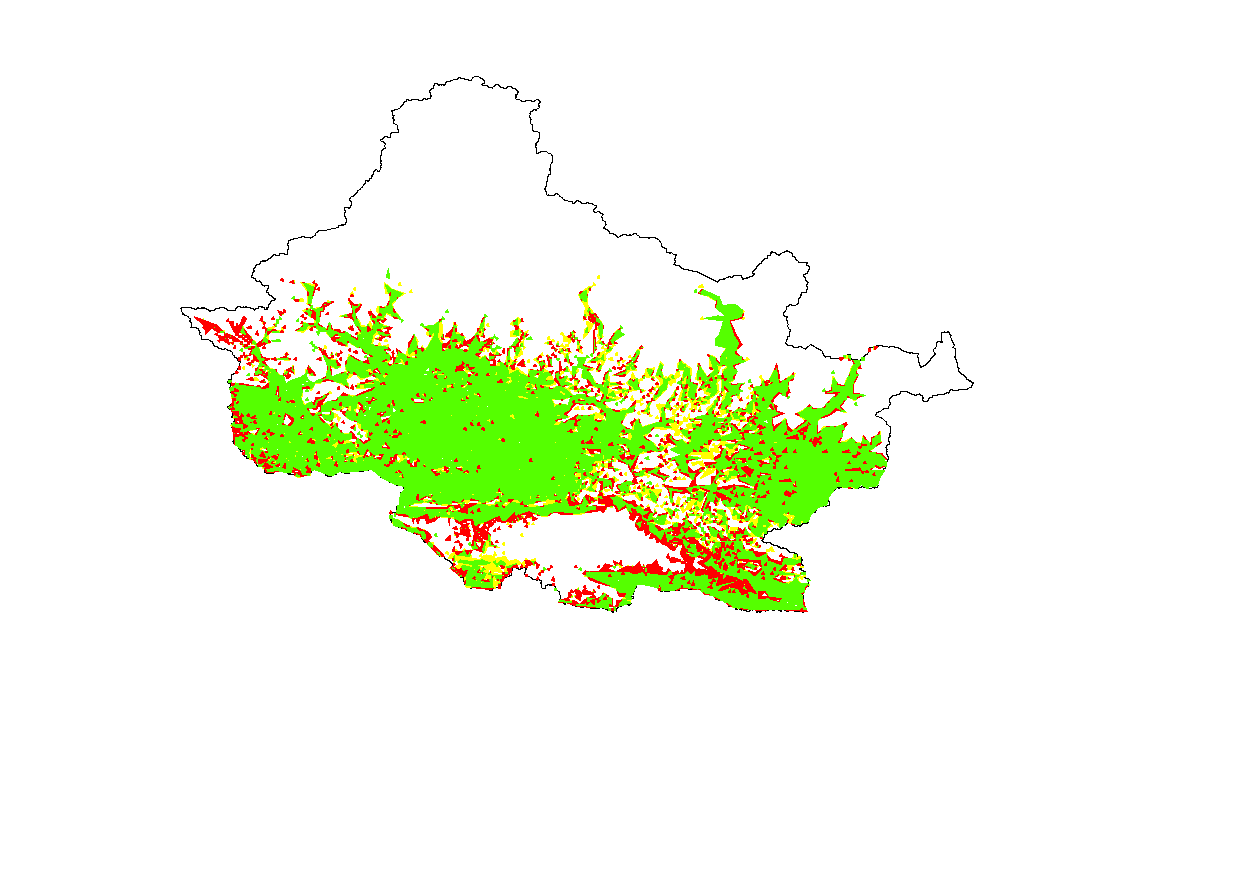
\includegraphics[trim=0 80 0 0,clip,width=5cm]{8550.pdf}};
    \node (8570.pdf) at (2,-11) [label=below:g] {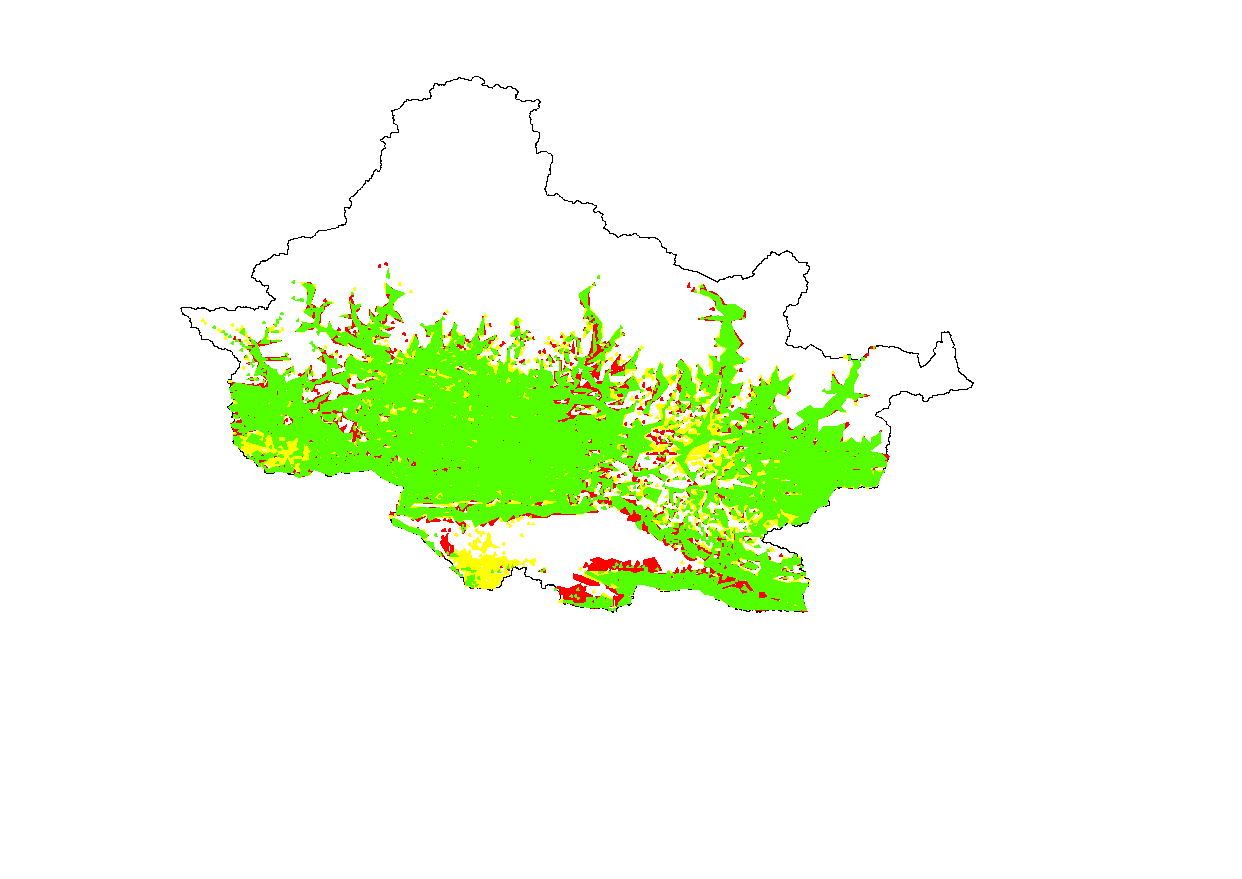
\includegraphics[trim=0 80 0 0,clip,width=5cm]{8570.pdf}};

%%
    \node at (-4,-1.8) {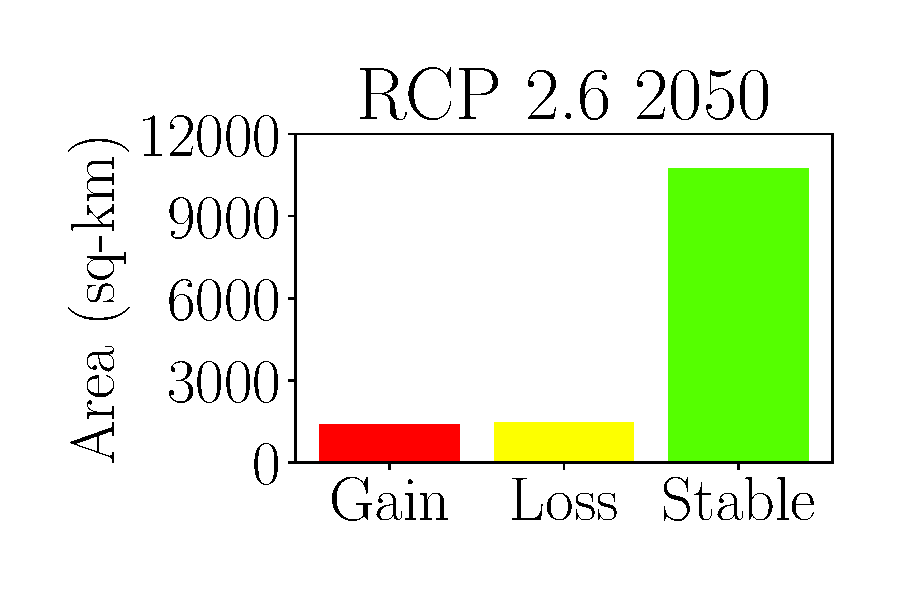
\includegraphics[trim=0 0 0 0,clip,width=2cm]{RCP_2.6_2050.pdf}};
    \node at (-4,-5.8) {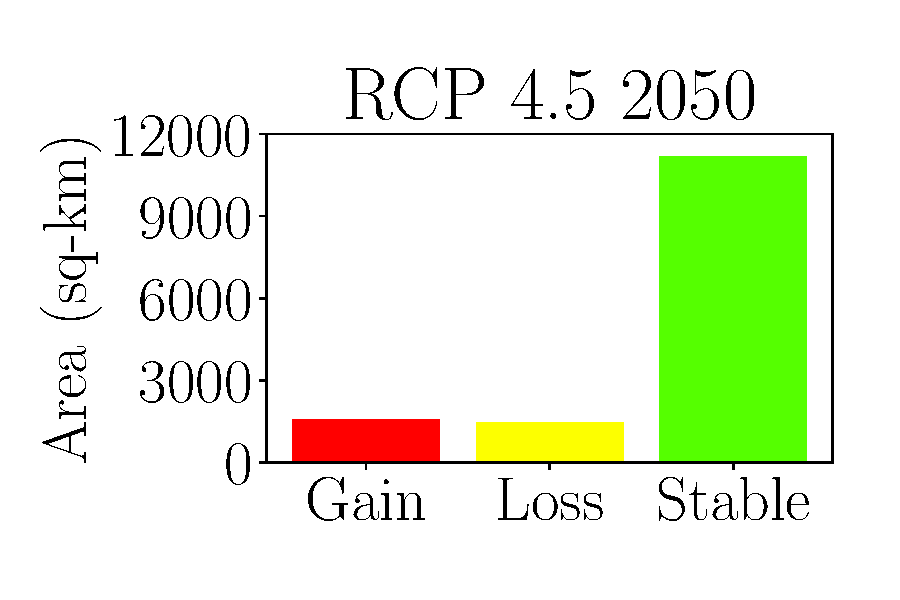
\includegraphics[trim=0 0 0 0,clip,width=2cm]{RCP_4.5_2050.pdf}};
    \node at (-4,-9.8) {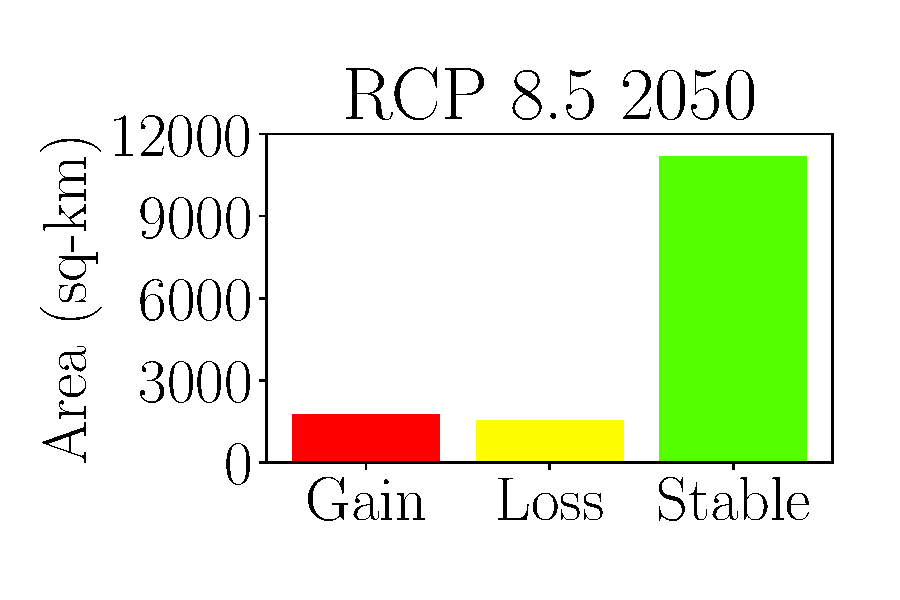
\includegraphics[trim=0 0 0 0,clip,width=2cm]{RCP_8.5_2050.pdf}};
%%
    \node at (3.5,-1.8) {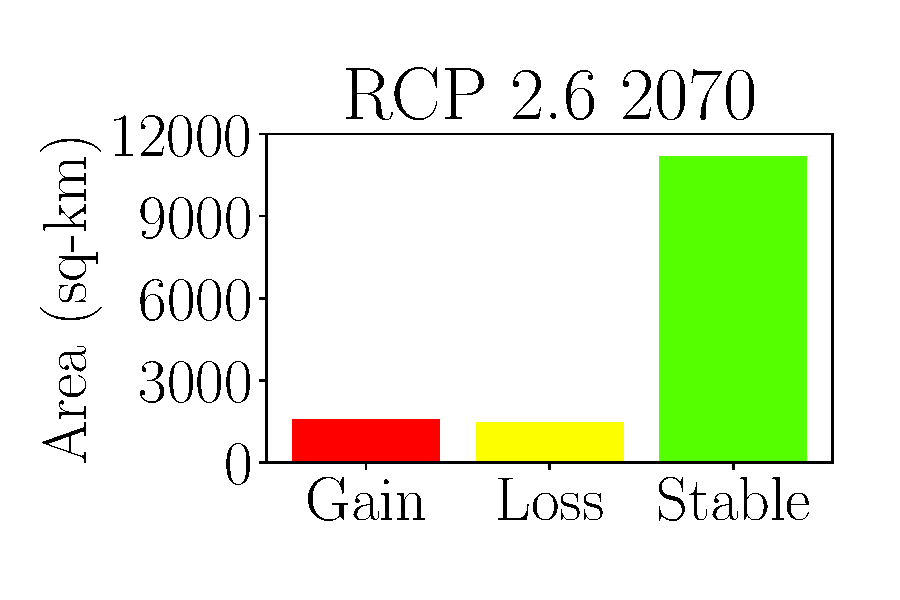
\includegraphics[trim=0 0 0 0,clip,width=2cm]{RCP_2.6_2070.pdf}};
    \node at (3.5,-5.8) {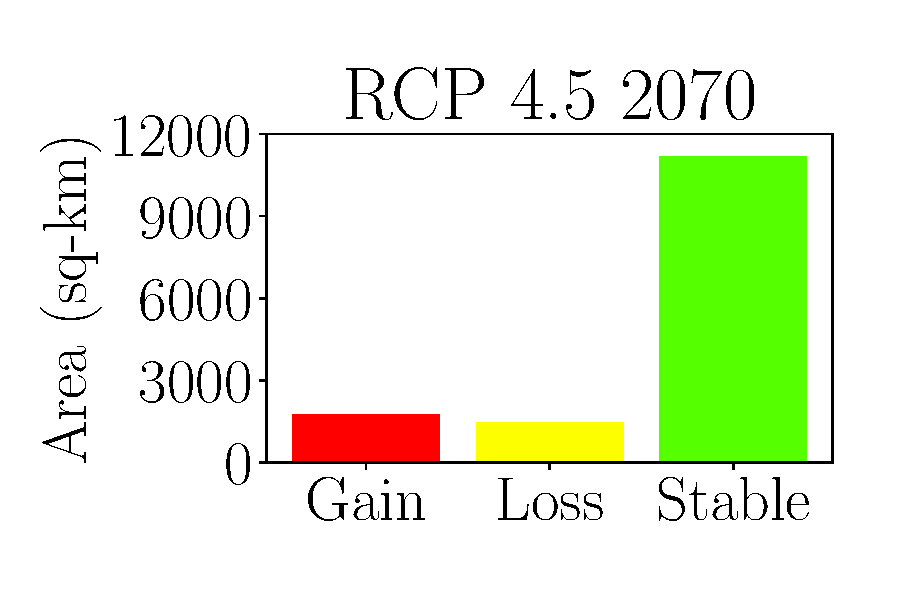
\includegraphics[trim=0 0 0 0,clip,width=2cm]{RCP_4.5_2070.pdf}};
    \node at (3.5,-9.8) {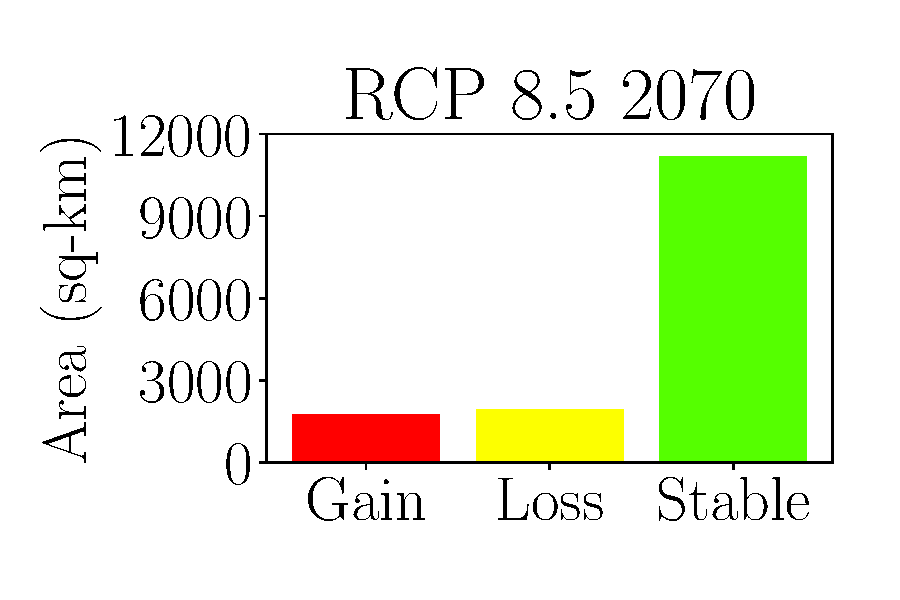
\includegraphics[trim=0 0 0 0,clip,width=2cm]{RCP_8.5_2070.pdf}};
\end{tikzpicture}
\end{document}
